%!TEX root = ../dissertation.tex

\begin{savequote}[75mm]
Nulla facilisi. In vel sem. Morbi id urna in diam dignissim feugiat. Proin molestie tortor eu velit. Aliquam erat volutpat. Nullam ultrices, diam tempus vulputate egestas, eros pede varius leo.
\qauthor{Quoteauthor Lastname}
\end{savequote}

\chapter{Background}

TODO

* object detector (theory)
* rnn + lstm
* textual embedding
* vocabulary (move to impl. details)

\section{Visual Grounding}

Visual grounding is the general task of locating the components of a
strucutred description in an image. Due to the ambiguous
interpretation of the general problem, it is usually decomposed in two
separated sub-problems, namely Referring Expression Grounding (REG)
and Phrase Grounding (PG).

\newthought{Referring Expression Grounding} is the simple task of
locating the subject referred by an expression in given image.

More formally, given in input an image $\bm{I}$ and a sentence
$\mathrm{S}$, REG consists in learning a function $\delta$ from the
set $\calS$ of sentences to a set of bounding boxes $B$ defined on
$\bm{I}$, i.e., $\delta: \calI \times \calS \rightarrow 2^{\calS
\times \calB}$, where $\calI$ is the domain of images, $\calS$ is the
domain of sentences, $\calB$ is the domain of bounding boxes which can
be defined on $\calI$, and $2^{\calS \times \calB}$ is the power set
of the cartesian product between $\calS$ and $\calB$.

\newthought{Phrase Grounding}, instead, is the task that studies the
mapping from noun phrases to regions of an image. In order to solve
this task, first, it is necessary to recognize all the objects in the
image and the components in the text, while after, the model needs to
find the correct alignment among the nouns and the objects.

More formally, given in input an image $\bm{I}$ and a sentence
$\mathrm{S}$, phrase grounding consists in learning a mapping $\gamma$
from the set $\calQ$ of noun phrases to a set of bounding box $\calB$
defined on $\bm{I}$, i.e., $\gamma : \calI \times \calS \rightarrow
2^{\calQ \times \calB}$. So, given an image $\bm{I}$ containing $e$
objects identified via the set of bounding boxes $B_\calI = \{ b_i
\}^e_{i=1}$, where $b_i \in \Rset^4$ is the vector of coordinates
identifying a bounding box in $\bm{I}$, and a sentence $\mathrm{S}$
containing $m$ noun phrases gathered in the set $\calQ_S = \{ q_j
\}^m_{j=1}$, where $q_j \in \Nset^2$ is a vector containing as
coordinates the initial and final character positions in the sentence
$\mathrm{S}$, $\gamma(\bm{I}, \mathrm{S})$ returns a set of couples
$\{ (\bm{q}, \bm{b}) \mid \bm{q} \in \calQ_{\mathrm{S}}, \bm{b} \in
B_{\bm{I}} \}$ where each couple $(\bm{q}, \bm{b})$ associates the
noun phrase $\bm{q}$ to the bounding box $\bm{b}$. Please, notice that
the same noun phrase can be associated to several different bounding
boxes, as well as the same bounding box can be associated to many
different noun phrases. Following the current literature, in this
paper we assume that each noun phrase is associated to one and only
one bounding box. Bounding boxes, however, can identify more objects,
e.g. several persons in the case the noun phrase is ``people''.

\newthought In of our work we will focus on phrase grounding, as it is
considered the foundamental building block for many high-level
computer vision tasks such as image retrieval, QA, video QA, etc.
\todo{remove from here} \todo{cite kwnowledge aided consistency}.

\cite{conser2019revisiting} \todo{FIX CITE}

\section{Two Stage vs One Stage}
\label{sec:two-stage-vs-one-stage}

Visual grounding is a challenging task which requires the semantic
understanding of the image content and its textual description. In
order to lower the complexity of the whole task, visual grounding is
generally formulated as an object detection task followed by a
classification task in which, given an input image and sentece, the
goal is to return only the detected object(s) that represents the best
semantic match with the sentence. This approach was extensively used
by many researchers in visual grounding field \todo{CITE vedere fast
and accurate one-stage approach...} due to its simplicity. On the
other hand, some recent works started introducing the one stage
approach in which the object detection and the classification problem
are solved joinly, arguing this new architecture may lead to faster
and more accurate models.

\newthought{The two stage approach} is a simple approach to the visual
grounding task which relies on the decomposition of the main task in
two sub-tasks, namely object detection and classification. Given an
input image, the first step generates candidate regions using an
object proposal extractor such us Edge Boxes and Selective Search
\todo{CITE edge box, selective searcg} or by an object detector, such
us Faster R-CNN, Single Shot multibox Detector (SSD), or YOLO
\todo{CITE faster rcnn, ssd, yolo...}. The second step consists in
ranking this candidate regions, which hopefully capture the semantic
context, conditioned on a language query about the image. Practically,
this means that the model predicts, for each proposal bounding box, a
score that represents how much the content of the bounidng box is
likely to be referred by the sentence. Sometimes, models predict also
new coordintas for the best predicted proposal, in order to better fit
the visual content accordingly to the sentence semantic information.
\todo{Aggiungere schema che descrive l'approccio}

Even if the approach seems very promising, it is not exempt from some
problems. As reported by \todo{CITE fast and acc one stage} ``the
propose-and-rank two stage framework is flawed in at least two major
ways''. First of all, if none of the region candidates of the first
stage hits the ground truth region, the whole framework fails no
matter how good the second ranking stage could perform. Note that a
hit is considered successful if any of the proposals overlap the
ground truth by more than fifty percent in term of intersection over
union (IoU). Secondly, they argue that the process can be optimized by
focusing on relevant bounding boxes which are often a small number
(2-5), instead of waste lot of resources by computing thousands of
proposal and then rank them down to a list.

However, the highlighted problems highly depends on chosen
proposal extractor/object detector. Consider, for example, the problem
of hitting the ground truth with at least one bounding box. Given an
image $\bm{I}$ and $b'$ the ground truth bounding box, if we employee
a very simple (yet extremely inefficient) proposal extractor such us
the one who generates $\bm{B}$ the set of all possible bounding boxes
in $\bm{I}$, then, by construction we have that $b' \in \bm{B}$. So,
by chosing the maximum number of bounding box we can tackle the
problem. However, this solution is not feasible in practice, but
fortunately we do not need to generate all possible solutions. In
fact, only a small subset of all solution are required to hit the
ground truth bounding box because thanks to the advancements in object
detection system we can recognize relevant objects in image and focus
only on those proposals.

Practically, we proved that with 100 bounding boxes and Faster-R CNN
object detector, we obtain a coverage which is greater than 90\% on
both two major dataset in the field of study: Flickr30k and ReferIt.
The table \todo{REF table} shows how the upperbound accuracy changes
by varying the number of considered bounding box.

The second problem instead is partially solvable because the system,
in order to perform its classification task, needs to consider all the
extracted proposal. However, the first stage can be precalculated and
cached for the second stage, drastically reducing the required
resources. 

\newthought{The one stage approach} firstly introducted by \todo{CITE
fast and accurate one stage}, instead, relies on a single step for
computing the solution. The model receives in input an image and a
textual sentence, and it should learn how to extract and fuse all the
visual and textual information in order to predict the best bounidng
box in output, according to the input sentence. 

The thight coupling provided by this approach may lead to interesting
results \todo{CITE fast and accurate one stage}, but it raises some
major issues: \begin{enumerate*}[label=(\roman*)] \item not all the
visual grounding datasets are suitable for training an object
detector, due to lack of images and/or because they are not densely
annotated; \item the model requires an high number of parameters, and
because of that \item the training requires significant computing
resources. \end{enumerate*}

\section{Fully/Weakly/Self/Un-Supervised Settings}

Machine learning has achieved great success in various tasks,
particularly in supervised learning tasks such as classification and
regression, but it is noteworthy that in many other tasks it is
difficult to get strong supervision information like fully
ground-truth labels due to the high cost of the data-labeling process.

Visual grounding is a striking example of that. Consider again the
example with image given in Fig.~\ref{img} and the sentence "A
colly..." \todo{completare sentence copiandola da sopra}.
\todo{Valutare se cambiare esempio o meno} In order to properly
evaluate the phrase localization task, is required to know each query
$q$ \todo{aggiustare matematica} in sentence $S$, and for each query
$q$ the mapping to a bounding box $b$ in image $I$, which means to
know also bounding boxes.\todo{aggiustare forma}. Practically
speaking, a human annotator given an image $I$ and a sentence $S$ has
to annotate all queries in sentence, undestand the query, identify the
referred object in image by drowing a bounding box surrounding it and
linking the bounding box with the query. With those insight it's
straighforward to see that the fully supervised scenario for the
visual grounding task is very hard to obtain. 

More abstractly, in fully supervised settings a training example
consists of two parts: a feature vector (or instance) describing the
event/object, and a label indicating the ground-truth output.
Projected in phrase grounding this means knowing the map $\gamma :
\calI \times \calS \rightarrow 2^{\calQ \times \calB}$ that links the
ground truth bounding box $b_i \in \calB$ with its query $q_j \in
\calQ$.

Another form of supervision is the weak supervision. Broadly speaking,
weakly supervised learning is an umbrella term covering a variety of
studiesthat attemptto construct predictive models by learning with
weak supervision \todo{CITE A brief introduction to weakly supervised
learning}. Typically, there are three types of weak supervision. 

\begin{itemize}
    \item The first is incomplete supervision, i.e. only a (usually
small) subset of training data is given with labels while the other
data remain unlabeled. \todo{AKA semi-supervised, CITE grounidng by
reconstruction}. Consider the following image TODO with the sentence
TODO \todo{}, in incomplete supervision we may lack some ground truth,
i.e., not for some query $q$, $\gamma(\bm{I}, S)$ is undefined.
    \item The second type is inexact supervision, i.e. only
coarse-grained labels are given. In phrase grounding inexact
supervision means we have weak ground truth, for example given
$\bm{I}$ an image and $S$ a sentence a weak ground truth may be the
map $\gamma' : \calI \times \calS \rightarrow 2^{\calI \times \calS}$.
Note that in this setting we do not know which bounding box $b$ is
linked to query $q$. \todo{aggiustare notazione math}
    \item The third type is inaccurate supervision, i.e. the given
labels are not always ground truth.  In other words, some label
information may suffer from errors.
\end{itemize}

The third type of weakly supervision in phrase grounding is usually
mixed with the other because the label procedure which must be carried
out by an human annotator and it's very error prone.

\section{NLP and Part of Speech Tagging}

Part of Speech (POS) Tagging is a very basic and well known Natural
Language Processing (NLP) problem which consists of assigning to each
word of a text the proper morphosyntactic tag in its context of
appearance \cite{marquez2000machine}. It is very useful for a number
of NLP applications: as a preprocessing step to syntactic parsing,
in information extraction and retrieval (e.g. document classification
in internet searchers), text to speech systems, corpus linguistics,
etc. The base of POS tagging is that many words being ambiguous
regarding their POS, in most cases they can be completely
disambiguated by taking into account an adequate context. Furthermore,
there are even cases in which the ambiguity is non-resolvable using
only morphosyntactic features of the context, and require semantic
and/or pragmatic knowledge. For instance, in the sample sentence
``Yesterday I read the paper'' the word \textit{read} is disambiguated
as a past simple because the word \textit{yesterday} at the beginning
of the sentence. Without context, the POS tagger can tag \textit{read}
also as a present or past participle.

Starting with the pioneer tagger \textsc{Taggit} developed by B. B.
Greene \etal{} in 1971, used for an initial tagging of the Brown
Corpus (BC), a lot of effort has been devoted to improving the quality
of the tagging process in terms of accuracy and efficiency. Existing
taggers can be classified into three main groups according to the kind
of knowledge they use: linguistic, statistic and machine-learning
family. Of course some taggers are difficult to classify into these
classes and hybrid approaches must be considered. Within the
linguistic approach most systems codify the knowledge involved as a
set of rules (or constraints) written by linguists. The linguistic
models range from a few hundreds to several thousand rules, and they
usually require years of labor.

The most extended approach nowadays is the statistical family
(obviously due to the limited amount of human effort involved).
Basically it consists of building a statistical model of the language
and using this model to disambiguate a word sequence. The language
model is coded as a set of co-occurrence frequencies for different
kinds of linguistic phenomena. This statistical acquisition is usually
found in the form of n-gram collection, that is, the probability of a
certain sequence of length $n$ is estimated from its occurrences in
the training corpus. In the case of POS tagging, usual models consist
of tag bi-grams and tri-grams (possible sequences of two or three
consecutive tags, respectively). Once the n-gram probabilities have
been estimated, new examples can be tagged by selecting the tag
sequence with highest probability. This is roughly the technique
followed by the widespread Hidden Markov Model taggers. Although the
form of the model and the way of determining the sequence to be
modeled can also be tackled in several ways, most systems reduce the
model to unigrams, bi-grams or tri-grams. Moreover, some taggers try
to reduce the amount of training data needed to estimate the model,
and use the Baum-Welch re-estimation algorithm. Other works that can
be placed in the statistical family performs energy-function
optimization using neural nets. Recent works in this field try not to
limit the model to a fixed order n-gram by combining different order
n-grams, morphological information, long-distance n-grams, or
triggering pairs. These are some approaches that we may see
incorporated to POS tagging tasks in the short term.

Although the statistical approach involves some kind of learning,
supervised or unsupervised, of the parameters of the model from a
training corpus, we place in the machine learning family only those
systems that include more sophisticated information than a n-gram
model. Many approaches were explored in literature: some works tried
to automatically learn a set of transformation rules which best repair
the errors committed by a most-frequent-tag tagger. Others acquire
Constraint Grammar rules from tagged corpora or apply instance-based
learning. Promosing approaches explore decision trees induced from
tagged corpora, which are exploited, together with other statistical
and linguistic information, in a hybrid environment that applies
relaxation techniques over a set of constraints.

\subsection{POS tags}

POS tags were originially defined in \cite{marcus1993building} on the
Penn Treebank corpus as a comprehensive list of tags for words,
including noun, adjective, verb tenses and also symbols. The
Fig.~\ref{fig:pos-tags} shows the tags along with their description.

\begin{figure}
  \centering
  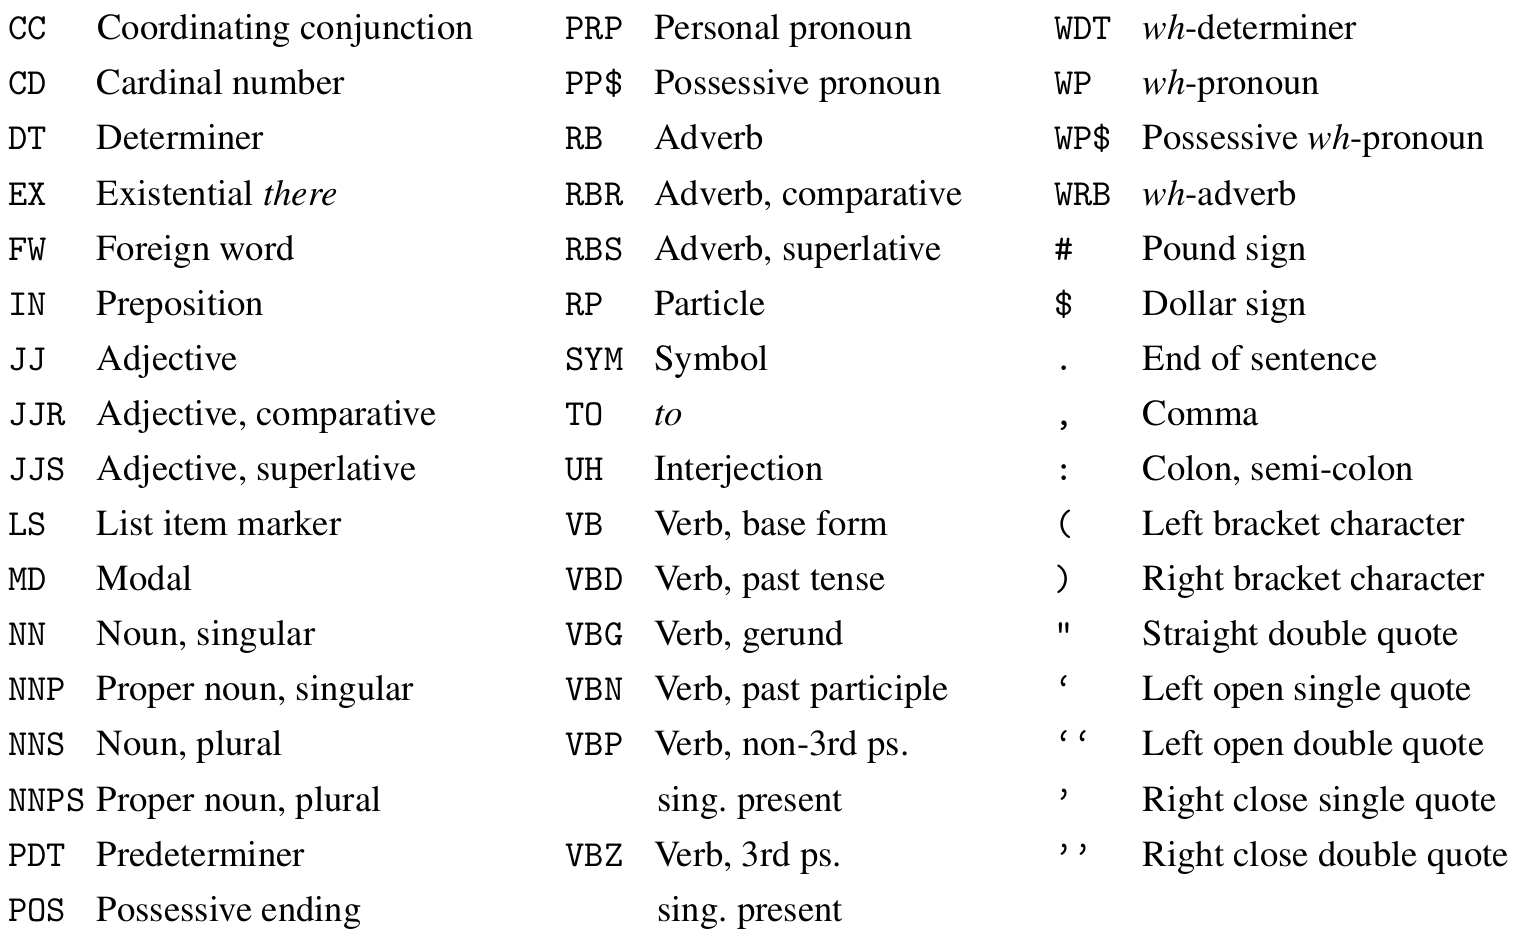
\includegraphics[width=.8\textwidth]{figures/pos-tags.png}
  \caption[POS tags]{POS tags of the Penn Treebank tag set \cite{marcus1993building}}
  \label{fig:pos-tags}
\end{figure}

During years, three different annotation standard of POS tagging and
dependency structure, such us Stanford Dependencies
\cite{de2006generating, de2008stanford, silveira2014gold}, Google
universal part-of-speech tags \cite{lin2012syntactic} and the Interset
interlingua \cite{zeman2008reusable} for morphosyntactic tagsets.
Universal Dependencies (UD) \cite{nivre2016universal,
nivre2017universal} is a recent effort to to achieve cross-linguistic
consistency of annotation, while still permitting language-specific
extensions when necessary. The UD annotation scheme uses a
representation in the form of dependency trees as opposed to a phrase
structure trees and makesavailable over $100$ treebanks of more than
$70$ languages. New Universal POS tags are listed in
Fig.~\ref{fig:upos-tags}.

\begin{figure}
  \centering
  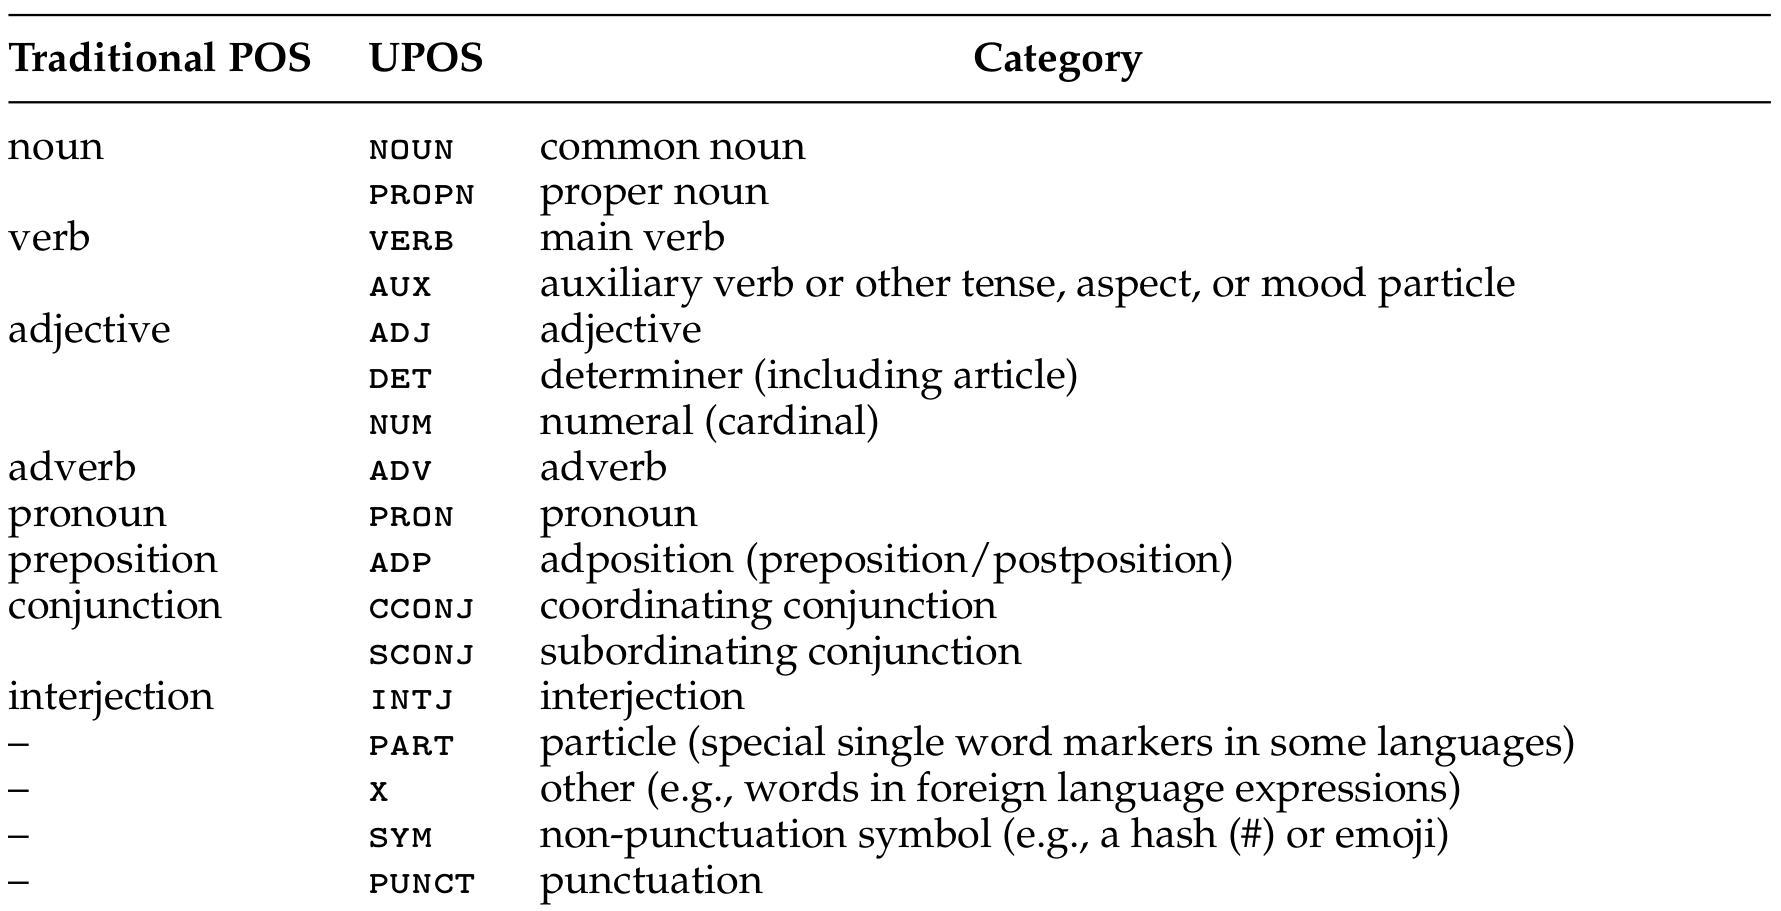
\includegraphics[width=.8\textwidth]{figures/upos-tags.png}
  \caption[Universal POS tags]{Universal part-of-speech tags (UPOS) \cite{nivre2017universal}}
  \label{fig:upos-tags}
\end{figure}
 
\section{Recurrent Neural Network}

A recurrent neural network (RNN) is a special type of an artificial
neural network (ANN) adapted to work for time series data or data that
involves sequences. Ordinary feed forward neural networks are only
meant for data points independent of each other while RNN introduces
the concept of ``memory'' that helps them store the states or
information of previous inputs to generate the next output of the
sequence by sharing weights.

An ANN with recursion can be easily modeled by the Eq.\ref{eq:rnn}:

\begin{equation}
  \label{eq:rnn}
  \bm{h}^{(t)} = f ( \bm{h}^{(t - 1)}, \bm{x}^{(t)} ; \bm{\theta} ),
\end{equation}

where $\bm{x}^{(1)}, \ldots, \bm{x}^{(\tau)}$ is the input sequence,
$f$ is the function that maps hidden units at time step $t - 1$ to
time step $t$ and $\bm{\theta}$ the parameters of $f$. The equation is
recurrent because the definition of $\bm{h}$ at time $t$ refers back to
the same definition at time $t - 1$. The process is visually depicted
in Fig.\ref{fig:rnn-with-unfold} \emph{(Left)} where the black square
indicates a delay of a single time step. At this point the problem is:
how do we propagate our input throught the RNN? Here comes in the idea
of unfolding. To unfold an RNN basically means to unroll the cyclic
circuit in a graph by explicitly applying the function $f$ on
$\bm{x}^{(t)}$, the input at time $t$, and $\bm{h}^{(t-1)}$, the
hidden state at time $t - 1$. RNN unfolding is visually explained in
Fig.\ref{fig:rnn-with-unfold} \emph{(Right)}.

\begin{figure}
  \centering
  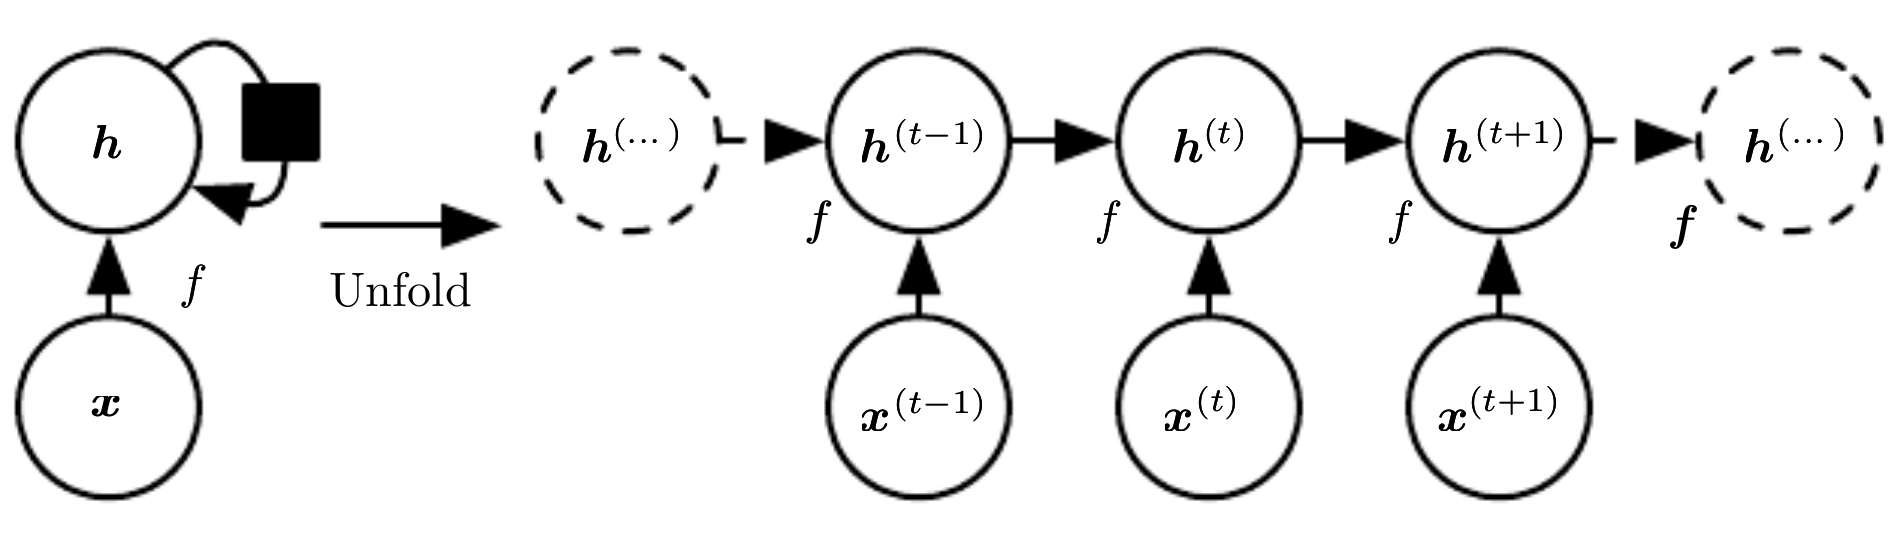
\includegraphics[width=.8\textwidth]{figures/rnn-with-unfold.png}
  \caption[TODO]{TODO: desc}
  \label{fig:rnn-with-unfold}
\end{figure}

Tipycal RNNs add extra architectural features such as output layers
that read information out of the state $\bm{h}$ to make predictions.

When the recurrent network is trained to perform a task that requires
predicting the future from the past, the network typically learns to
use $\bm{h}^{(t)}$ as a kind of lossy summary of the task-relevant
aspects of the past sequence of inputs up to t. This summary is in
general necessarily lossy, since it maps an arbitrary length sequence
$( \bm{x}^{(t)}, \bm{x}^{(t-1)}, \bm{x}^{(t-2)} , \ldots ,
\bm{x}^{(2)}, \bm{x}^{(1)} )$ to a fixed length vector $\bm{h}^{(t)}$ .
Depending on the training criterion, this summary might selectively
keep some aspects of the past sequence with more precision than other
aspects. For example, if the RNN is used in statistical language
modeling, typically to predict the next word given previous words, it
may not be necessary to store all of the information in the input
sequence up to time $t$, but rather only enough information to predict
the rest of the sentence.

Recurrent neural networks can be built in many different ways with
varying architecture. In literature emerged some successful RNNs
architecture with a well defined and non-casual structure, such us
Bidirection RNN (Bi-RNN), Long Short-Term Memory (LSTM) and Gated
Recurrent Unit (GRU). Each RNN architecture has some pro and cons and
can be applied successfully to specific tasks.

\subsection{Bidirectional RNN}

As the name suggests, bidirectional RNNs combine an RNN that moves
forward through time beginning from the start of the sequence with
another RNN that moves backward through time beginning from the end of
the sequence. Those networks have been applied successfully when the
output we want to predict depetnds on the whole input sequence. For
example, in speech recognition, the correct interpretation of the
current sound as a phoneme may depend on the next few phonemes because
of co-articulation and potentially may even depend on the next few
words because of the linguistic dependencies between nearby words: if
there are two interpretations of the current word that are both
acoustically plausible, we may have to look far into the future (and
the past) to disambiguate them. This is also true of handwriting
recognition and many other sequence-to-sequence learning tasks such us
bioinformatics.

The Bi-RNNs convoy an intrisic advantage and drawback at the same
time: it requires the full sequence, so it cannot work with real-time
input sequences, but for the same reason it can better infer the
output from the past and future kwown context.

\subsection{Gated RNN (LSTM and GRU)}
\label{subsec:gated-rnn}

Being able to work with long term dependencies is crucial for many
applications: think, for example, to a dialogue system which should
remember previous parts of the speech on order to keep on with the
dialogue.

Unfortunately, RNNs and long term dependencies yield a mathematical
challenge. The basic problem is that gradients propagated over many
stages tend to either vanish (most of the time) or explode (rarely,
but with much damage to the optimization). Moreover, I. Goodfellow
\etal{} in \todo{CITE: deeplearningbook}, states also that:

\begin{quote}
  Even if we assume that the parameters are such that the recurrent
  network is stable (can store memories, with gradients not
  exploding), the difficulty with long-term dependencies arises from the
  exponentially smaller weights given to long-term interactions
  (involving the multiplication of many Jacobians) compared to
  short-term ones.
\end{quote}

One way to deal with long-term dependencies is to design a model that
operates at multiple time scales, so that some parts of the model
operate at fine-grained time scales and can handle small details, while
other parts operate at coarse time scales and transfer information
from the distant past to the present more efficiently. Various
strategies for building both fine and coarse time scales are possible.
These include the addition of skip connections across time, ``leaky
units'' that integrate signals with different time constants, and the
removal of some of the connections used to model fine-grained time
scales.

Like leaky units, gated RNNs are based on the idea of creating paths
through time that have derivatives that neither vanish nor explode.
Leaky units did this with connection weights that were either manually
chosen constants or were parameters. Gated RNNs generalize this to
connection weights that may change at each time step.

Leaky units allow the network to accumulate information (such as
evidence for a particular feature or category) over a long duration.
However, once that information has been used, it might be useful for
the neural network to forget the old state. For example, if a sequence
is made of sub-sequences and we want a leaky unit to accumulate
evidence inside each sub-subsequence, we need a mechanism to forget
the old state by setting it to zero. Instead of manually deciding when
to clear the state, we want the neural network to learn to decide when
to do it.

LSTM basically integrates the idea of self-loops to produce paths
where the gradient can flow for long durations with the addition to
control weight on this self-loop conditioned on the context, rather
than fixed. By making the weight of this self-loop gated (controlled by
another hidden unit), the time scale of integration can be changed
dynamically. LSTM recurrent networks have ``LSTM cells''that have an
internal recurrence (a self-loop), in addition to the outer recurrence
of the RNN. Fig.~\ref{fig:lstm} illustrate the LSTM block diagram. In
an LSTM cell, the self-loop controls the flow of information from
input to output through three key components: a forget gate, an
external input gate and an output gate.

\begin{figure}
  \centering
  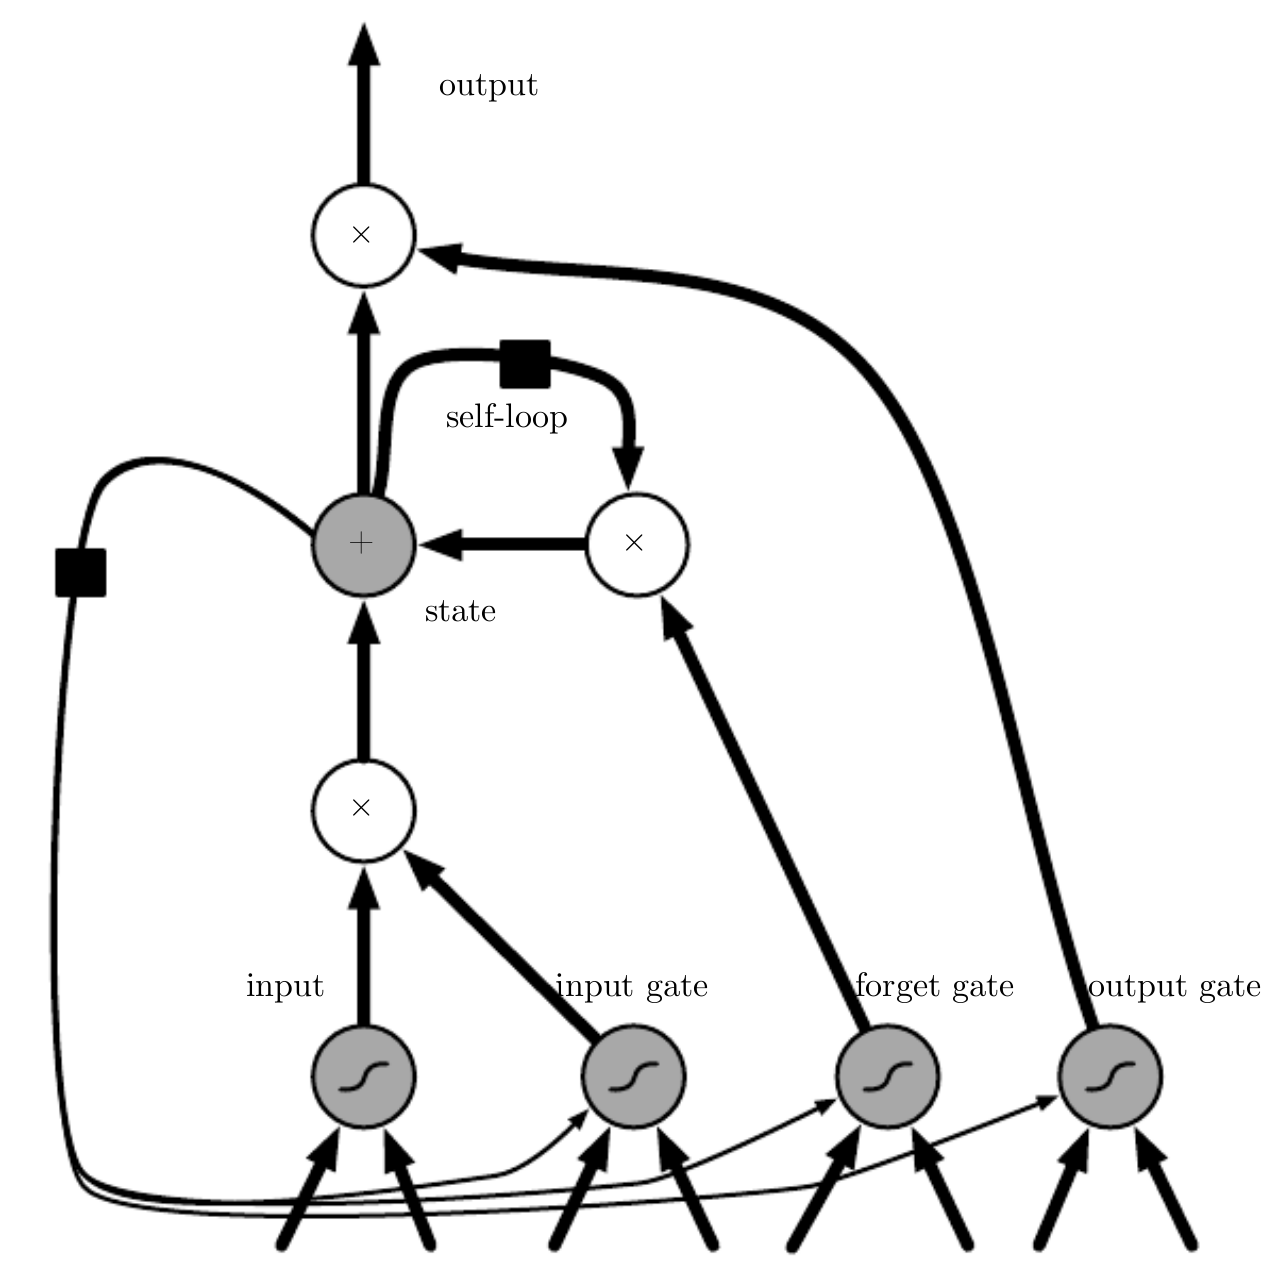
\includegraphics[width=.6\textwidth]{figures/lstm.png}
  \caption[TODO]{TODO: desc}
  \label{fig:lstm}
\end{figure}

Along with LSTM architecture, a simpler version was recently proposed
with the aim to simplify cells and speed-up computations: the gated
recurrent units (GRU). The behaviour wrt LSTM is very similar, the
only difference is that a single gating unit simultaneously controls
the forgetting factor and the decision to update the state unit.

\section{Object Detection and Recognition Systems}
\label{sec:object-detection-recognition}

Object detection (OD) and object recognition (OR) systems are crucial
in a wide variety of everyday tasks such us face detection, image and
video databases information retrieval, surveillance applications,
driver assistance, self drive, robotics, automation and, specially in
vision tasks, it is a foundamental building block used to extract
information from images.

The primary essence of those systems can be broken down into two
parts: to locate objects in a scene such us by drawing a bounding box
around the object (object detection) and later to classify the objects
based on the classes it was trained on (obejct recognition). OD and OR
are Often used together and for this reason the name of two tasks is
usually used interchangeably. As for visual grounding
(Sec.~\ref{sec:two-stage-vs-one-stage}), we can group the
state-of-the-art detection systems in two main approaches: one stage
methods (YOLO - You Only Look Once \todo{CITE: yolo}, SSD - Single
Shot Detection \todo{CITE: ssd}) and two stage methods (R-CNN, Fast
R-CNN, Faster R-CNN \todo{CITE: RCNN}). 

In the following sections, we briefly summarize those methods
discussing their main idea nd highlighting pro and cons.

\subsection{YOLO -- \emph{You Only Look Once}}

YOLO is a state-of-the-art, real-time object detection system which
offers extreme levels of speed and accuracy. YOLO reframes object
detection as a regression problem to spatially separated bounding
boxes and associated class probabilities. A single neural network
predicts bounding boxes and class probabilities directly from full
images in one evaluation. Since the whole detection pipeline is a
single network, it can be optimized end-to-end directly on detection
performance. This architecture offers some advantages wrt to other
methods: first, YOLO is extremely fast and second, it reasons globally
about the image when making prediction implicitly encoding contextual
information about classes as well as their appearance. Last but not
least, YOLO is more likely to learn generalizable representations of
objects because of its global reasoning on image.

\subsection{SSD -- \emph{Single Shot Detection}}

SSD is another state-of-the-art method for detecting objects in images
using a single deep neural network. SSD discretizes the output space
of bounding boxes into a set of default boxes over different aspect
ratios and scales per feature map location and, at prediction time,
the network generates scores for the presence of each object category
in each default box and produces adjustments to the box to better
match the object shape. Additionally, the network combines predictions
from multiple feature maps with different resolutions to naturally
handle objects of various sizes. Also, SSD offers high speed
performance due its single network and for this reason it is easy to
train and straightforward to integrate into systems that require a
detection component. In terms of accuracy, experimental results confirm
that SSD has competitive accuracy also in low resolution compared to
methods that utilize an additional object proposal step.

\subsection{R-CNN -- \emph{Regions with CNN}}

R-CNN is the first performant object detection system ever built. It
is composed by a two-stage architecture: in the first step the
Selective Search algorithm generates around 2000 category-independent
region proposals for the input image, in the last step instead it
extracts a fixed-length feature vector from each proposal using a CNN
(hence the name R-CNN), and then classifies each region with
category-specific linear SVMs. The method shows interesting results
and can be applied also with scarce data availability: the system can
be pretrained and the fine-tuned. In temrs of computation time, R-CNN
performs some expensive operations required for greedy non-maximum
suppression, amogn others, but on relatively small inputs.

\subsection{Fast R-CNN}

The Fast R-CNN model was built to counter a few drawbacks of the
previous R-CNN model. In this approach, similar to the previous,
Selective Search is used to generate region proposals but the input
image is fed to a CNN and a convolutional feature map is generated
from it which is then used to identify the regions and combine them
into larger squares by using a RoI pooling layer. A softmax layer is
finally used to predict the class of the proposed region.

\subsection{Faster R-CNN}

Unlike R-CNN and Fast R-CNN, Faster R-CNN does not use Selective
Search which is a slow process. Instead, it allows the network to
learn the region proposals throught a separate network, able to
predict the region proposals. The predicted proposals are then pooled
into larger squares using the RoI pooling layer which is then finally
used to classify the image.

\todo{ADD: quale abbiamo scelto? attenzione a quanto già detto in introduzione (potrebbe essere spostato qui...)}

\section{Word Embeddings}
\label{sec:word-embeddings}

Being able to model and represent natural language features is a
relevant machine learning task that belongs to the natural language
processing field and has many applications, such us information
retrieval (Manning et al., 2008), document classification (Sebastiani,
2002), question answering (Tellex et al., 2003), named entity
recognition (Turian et al., 2010), and parsing (Socher et al., 2013).
\todo{CITE: recupeare i paper dal paper GloVe} 

Instead of treating words as atomic units where there is no notion of
similarity between words, as these are represented as indices in a
vocabulary, natural language information can be represented as
real-valued feature vectors throught a semantic vector space, where
representation of words are learned for a predefined fixed sized
vocabulary from a corpus of text and the intrinsic quality of such a
set of word is evaluated by the distance or angle between pairs of
word vectors representations or by their various dimensions of
difference\todo{CITE:  Mikolov et al. (2013c)}. In light of this we
can formulate the definition for word embedding: 

\begin{quote}
    \textit{A word embedding is a learned representation for text
    where words that have the same meaning have similar
    representation.}
\end{quote}

With the years, literature explored different approaches for learning
good words representation: either joint with the neural network model
on some task, such as document classification, or using document
statistics throught unsupervised settings.

\subsection{Indexing by Latent Semantic Analysis}

A first approach for learning representative word embeddings was first
introduced by S. Deerwester \etal{} in \todo{CITE: Deer- wester et
al., 1990}, exploiting global matrix factorization by means of latent
semantic analyis (LSA). The proposed approach tries to overcome the
deficiencies of term-matching retrieval by treating the unreliability
of observed term-document association data as a statistical problem.
Indeed, they take advantage of a particular version of LSA that uses
singular-value decomposition. First, a large matrix of term-document
association data is crteated and then a semantic space wherein terms
and documents that are closely associated are placed near one another
is constructed. Singular-value decomposition allows the arrangement of
the space to reflect the major associative patterns in the data, and
ignore the smaller, less important influences.

\subsection{Word2Vec}

Word2Vec, introduced by T. Mikolov in \todo{CITE: w2v-1} and then
updated and revisioned in \todo{CITE: w2v-2, w2v-3}, is a statistical
method for efficiently learning a standalone word embedding from a
text corpus. One of the goal of Word2Vec is to learn distributed
representations of words by neural networks, in particular, they
introduced two different learning models that can be used as part of
the word2vec approach to learn the word embedding: Continuous
ag-of-Words (CBOW) and Continuous Skip-Gram Model. The CBOW model
learns the embedding by predicting the current word based on its
context. The continuous skip-gram model learns by predicting the
surrounding words given a current word. Both models, shown in
Fig.~\ref{fig:word2vec-learning-models} are focused on learning about
words given their local usage context, where the context is defined by
a window of neighboring words. This window is a configurable parameter
of the model. The quality of these representations is measured in a
word similarity task.

\begin{figure}
  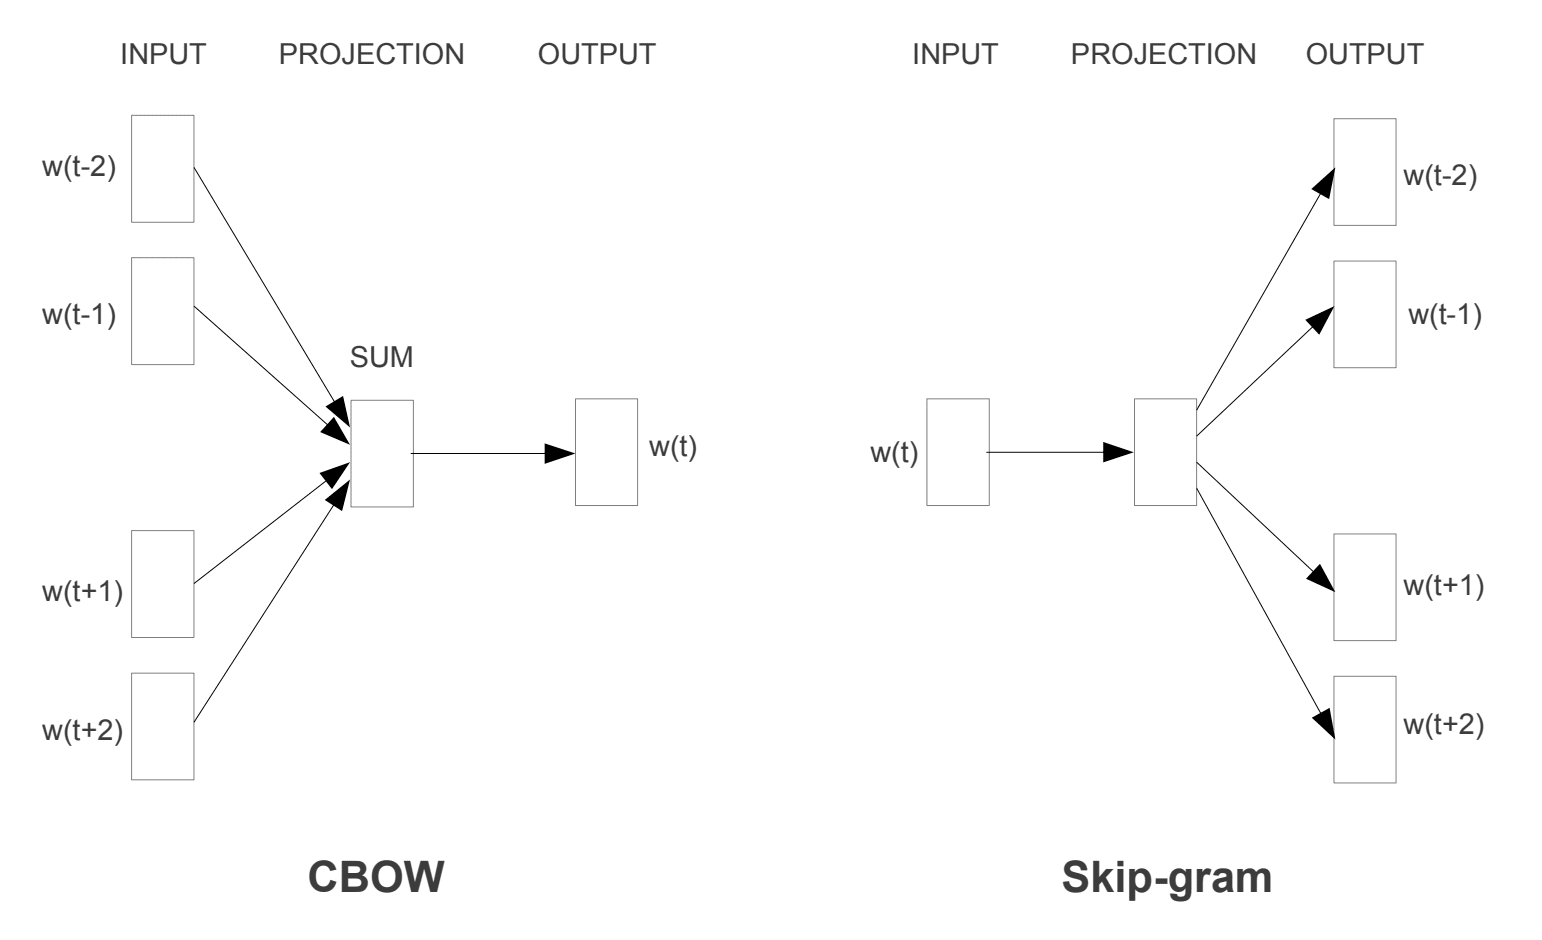
\includegraphics[width=\textwidth]{figures/word2vec-training-models.png}
  \caption[TODO]{TODO: desc}
  \label{fig:word2vec-learning-models}
\end{figure}

The key benefit of the approach is that high-quality word embeddings
can be learned efficiently (low space and time complexity), allowing
larger embeddings to be learned (more dimensions) from much larger
corpora of text (billions of words). Also, Word2Vec perform
significantly better than LSA for preserving linear regularities among
words and LDA moreover becomes computationally very expensive on
large data sets.

\subsection{GloVe}

GloVe is an extension to the Word2Vec method for efficiently learning
word vectors, developed by Pennington \etal{} in \todo{CITE: glove},
that wants to to marry both the global statistics of matrix
factorization techniques like LSA with the local context-based
learning in Word2Vec. Rather than using a window to define local
context, GloVe constructs an explicit word-context or word
co-occurrence matrix using statistics across the whole text corpus.
The result is a learning model that may result in generally better
word embeddings.

\subsection{Other methods}

\newthought{BERT} -- Bidirectional Encoder Representations from Transformers is a relatively recent language representation model, introduced by J. Devlin \etal{} in \todo{CITE: BERT: Pre-training of Deep Bidirectional Transformers for Language Understanding},  designed to pretrain deep bidirectional representations from
unlabeled text by jointly conditioning on both left and right context in all layer. BERT’s key technical innovation is applying the bidirectional training of Transformer, a popular attention model, to language modelling. This is in contrast to previous efforts which looked at a text sequence either from left to right or combined left-to-right and right-to-left training.

\todo{ADD OR REMOVE: Both families suffer significant drawbacks. While methods like LSA efficiently leverage statistical information, they do relatively poorly on the word analogy task, indicating a sub-optimal vector space structure. Methods like skip-gram may do better on the analogy task, but they poorly utilize the statistics of the corpus since they train on separate local context windows instead of on global co-occurrence counts.}

\section{Similarity Measures}

\subsection{Intersection over Union (IoU)}

Given a pair of bounding box coordinates (b i , b j ), the
Intersection over Union (IoU), also known as Jaccard index, is an evaluation metric used mainly in object detection
tasks, which aims to evaluate how much the two bounding
box refer to the same content in the image. Specifically, it
is defined as:
\[
  \iou(\bbox_i, \bbox_i) = \frac{| \bbox_i \inters \bbox_j |}{| \bbox_i \union \bbox_j |}
\]
where $| \bbox_i \inters \bbox_j |$ is the area of the box obtained by
the intersection of boxes $\bbox_i$ and $\bbox_j$ , while $| \bbox_i
\union \bbox_j |$ is the area of the box obtained by the union of
boxes $\bbox_i$ and $\bbox_j$. It is invariant to the bounding boxes
sizes, and it returns values that are strictly contained in the
interval $[0, 1] \in \Rset$, where $1$ means that the two bounding
boxes refer to the same image area, while a score of $0$ means that
the two bounding boxes do not overlap at all. The fact that two
bounding boxes that do not overlap have IoU score equal to $0$, is the
major issue of this metric: the zero value does not represent how much
the two bounding boxes are far from each other. For this reason, in
its standard definition, the intersection over union is mainly used as
an evaluation metric rather than as a component of a loss function for
learning.

\subsection{Cosine Similarity}

Cosine similarity is a metric used to measure how similar
representations are irrespective of their size (norm). Mathematically,
it measures the cosine of the angle between two vectors projected in a
multi-dimensional space:
\begin{equation}
  s_{\cos}(\bm{a}, \bm{b}) = \frac{\veca \cdot \vecb}{\normtwo\veca \normtwo\vecb},
\end{equation}
where $\veca \cdot \vecb$ is the dot product between two vectors and
$\normtwo\veca$ is the L2-norm of a vector.
